\chapter{Datasets, Experimental Setup, and Baselines}
\label{ch:datasets_implementation}

Understanding the data is a prerequisite for successful modeling. This chapter analyzes the specific characteristics of the chosen datasets, defends their suitability, and establishes benchmarking protocols.

\section{Dataset Suitability and Defense}

To address the query about data set sufficiency, the project utilizes two of the most cited and rigorous datasets in the battery domain. Their specific characteristics, artifacts and strategic roles in this research are detailed in Table \ref{tab:datasets} below.

% --- TABLE 5.1: DATASET SPECIFICATIONS ---
\begin{table}[H]
\centering
\caption{Specification and Characteristics of Selected Datasets}
\label{tab:datasets}
\renewcommand{\arraystretch}{1.5} % Adds breathing room between rows
\small % Slightly smaller font to ensure fit
\setlength{\tabcolsep}{4pt}        % trim inter-column padding so the table clears the right margin
\begin{tabular}{|p{2.6cm}|p{1.7cm}|p{3.7cm}|p{3.7cm}|}
\hline
\textbf{Dataset \& Cell ID} & \textbf{Chemistry} & \textbf{Key Artifacts \& Noise} & \textbf{Role in Thesis} \\
\hline
\textbf{NASA PCoE} \newline (Cells B0005--B0007, B0018) & LiCoO$_2$ \newline (18650) & \textbf{Capacity Regeneration:} Significant ``jumps'' in capacity after rest periods (B0005 shows 36 such jumps, up to 0.088~Ah). A pure data-driven model might overfit this and predict ``healing.'' & \textbf{Noise Robustness:} Validates ``Physical Consistency.'' The Verhulst ODE enforces $\frac{dSOH}{dt} \leq 0$, testing if the model can ignore non-physical noise \cite{auto_regression_pf}. \\
\hline
\textbf{CALCE} \newline (Cell CS2\_35) & LiCoO$_2$ \newline (prismatic) & \textbf{Knee-Point:} Distinct acceleration in degradation after $\approx$650 cycles; a much longer life (878 cycles) and a different form factor and load profile than NASA. & \textbf{Generalizability:} Tests whether physics constraints help the model generalize across different operating conditions, loads, and form factors (cross-dataset, same chemistry) \cite{inheritance_pf}. \\
\hline
\end{tabular}
\end{table}

\noindent
\textbf{Note on chemistry.} Both datasets are LiCoO$_2$ (LCO) cells. The
NASA$\leftrightarrow$CALCE comparison is therefore a \emph{cross-dataset /
cross-load / cross-form-factor} test, \emph{not} a cross-chemistry one. (An earlier
draft described CALCE as LFP/NMC; direct inspection of the cells confirms LCO.)

\noindent
To illustrate the challenges these datasets present, Figures
\ref{fig:nasa_degradation} and \ref{fig:calce_timelines} visualize the distinct
degradation profiles. The NASA cells exhibit significant noise due to
regeneration, whereas CALCE shows a long, gradual fade with a late knee-point.

% --- FIGURE 5.1a: NASA DEGRADATION ---
\begin{figure}[H]
    \centering
        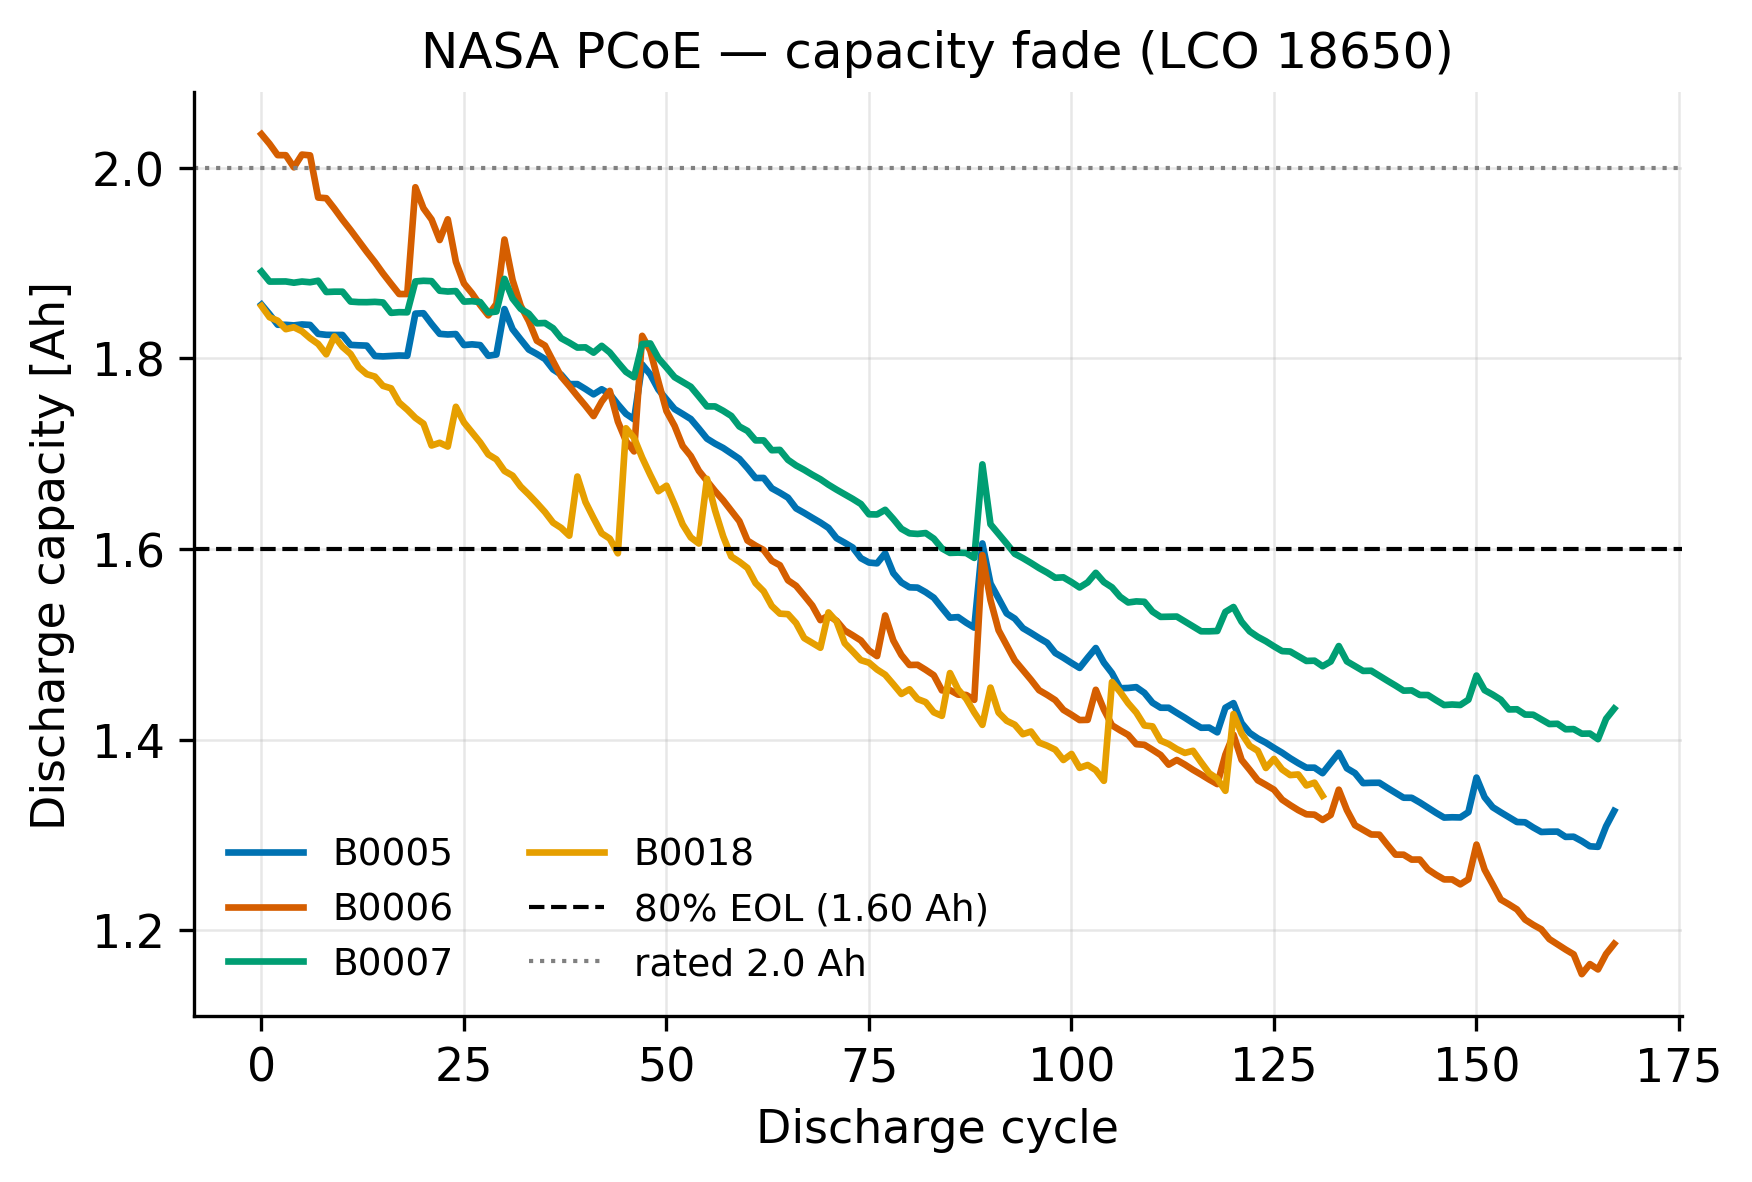
\includegraphics[width=0.8\textwidth]{2-mainmatter/chapters/nasa_degradation.png}
    \caption{NASA PCoE capacity fade for all four LCO 18650 cells over their true
    132--168 cycle lifetimes. Regeneration ``jumps'' after rest periods are visible
    as upward spikes; the dashed line marks the 80\% EOL (1.60~Ah) against the
    2.0~Ah rated capacity.}
    \label{fig:nasa_degradation}
\end{figure}

% --- FIGURE 5.1b: CALCE TIMELINES ---
\begin{figure}[H]
    \centering
        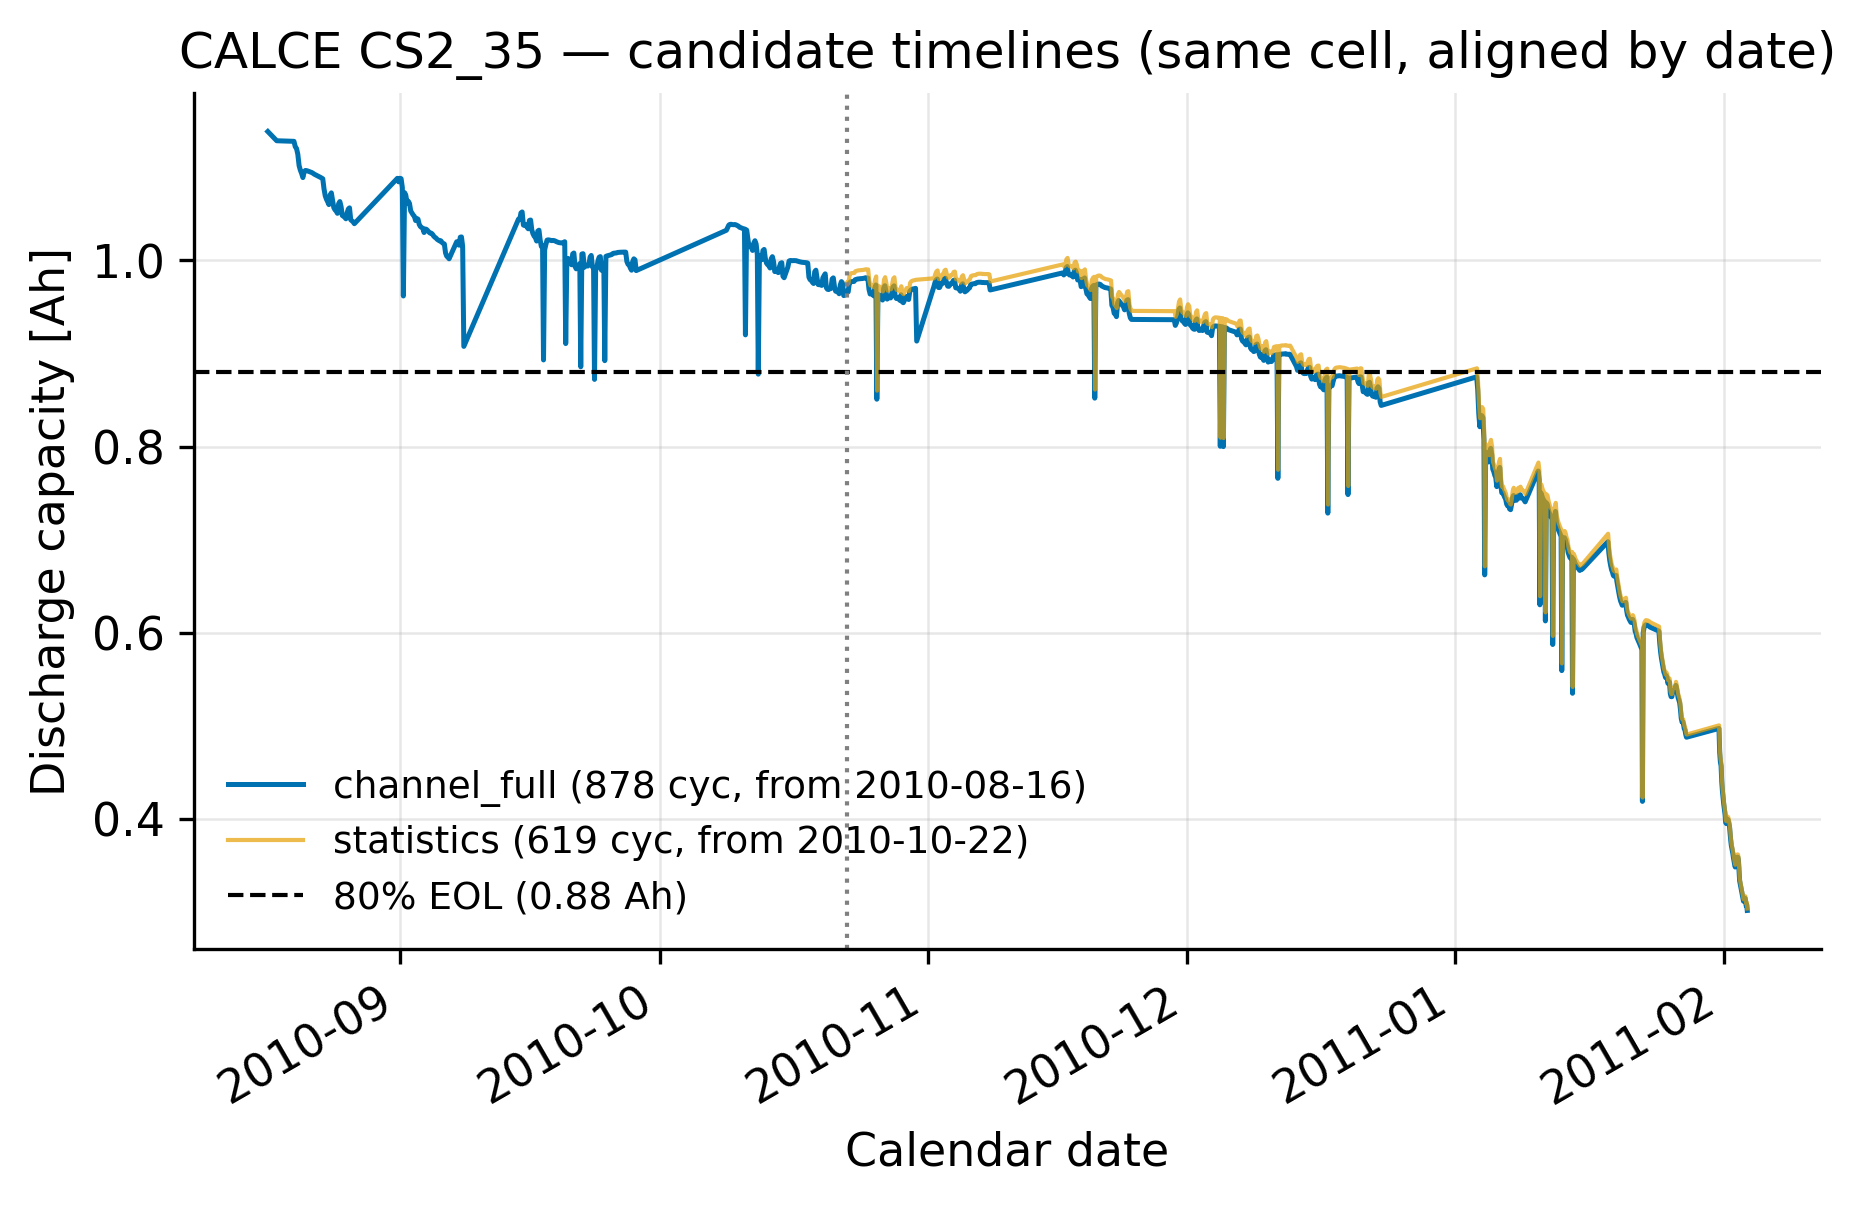
\includegraphics[width=0.8\textwidth]{2-mainmatter/chapters/calce_timelines.png}
    \caption{CALCE CS2\_35 candidate timelines (same physical cell, aligned by
    date). The \texttt{channel\_full} timeline (878 cycles from 2010-08-16,
    1.14$\rightarrow$0.30~Ah) is adopted; the \texttt{statistics} export is the same
    cell minus early life and is not used. The knee-point and 80\% EOL are marked.}
    \label{fig:calce_timelines}
\end{figure}

\noindent
\textbf{Exploratory Data Analysis (EDA):}
For NASA, the measured cycle counts are 168/168/168/132 (B0005/06/07/B0018); the
80\% EOL (with 5-cycle persistence) is reached at 58--93 cycles, and B0007 never
crosses the 70\% threshold within its record. CALCE CS2\_35 (\texttt{channel\_full})
runs 878 cycles and reaches 80\% EOL around cycle 585.

\textbf{Conclusion on Datasets:} These two datasets provide a comprehensive testbed
covering both ``noise robustness'' (NASA short-life cells with heavy regeneration)
and ``dynamic generalization'' (CALCE long-life cell, different load and form
factor), providing a sufficient and rigorous testbed for the present study.

% --- NEW CONTENT STARTS HERE ---
\subsection{Technical Data Breakdown and Preprocessing}
\label{subsec:technical_breakdown}

Based on the initial preprocessing pipelines, a detailed technical breakdown of the features, targets, and dimensionalities of both datasets has been established. This ensures that the neural network inputs are properly bounded and engineered for physical relevance. Table \ref{tab:feature_breakdown} provides a comparative summary of these engineered features.


\begin{table}[htbp]
\centering
\caption{Detailed Feature Breakdown of Processed Datasets}
\label{tab:feature_breakdown}
% \tabularx{TotalWidth}{ColumnTypes}
\begin{tabularx}{\textwidth}{@{} >{\raggedright\arraybackslash}p{0.22\linewidth} X X @{}}
\toprule
\textbf{Feature Category} & \textbf{NASA PCoE Dataset} & \textbf{CALCE Dataset} \\
\midrule
Batteries Profiled & B0005, B0006, B0007, B0018 & CS2\_35 (\texttt{channel\_full}, stitched from multiple date files) \\
Rated Capacity & 2.0 Ah & 1.1 Ah \\
Initial Capacity & 1.856 / 2.035 / 1.891 / 1.855 Ah & $\approx 1.14$ Ah (0.88 Ah is mid-life, not initial) \\
Cycles Extracted & 168 / 168 / 168 / 132 & 878 continuous cycles \\
Primary Target (Y) & per-cycle capacity $\rightarrow$ SOH $= Q/Q_\text{rated}$ (raw, unsmoothed) & per-cycle capacity $\rightarrow$ SOH $= Q/Q_\text{rated}$ (raw, unsmoothed) \\
\midrule
\textbf{Shared physics-informed features} & \multicolumn{2}{c}{\texttt{ica\_peak\_voltage\_V}, \texttt{ica\_peak\_magnitude}, \texttt{ica\_area} (from $dQ/dV$)} \\
\midrule
\textbf{Electrical / state features} & \multicolumn{2}{c}{\texttt{discharge\_time\_s}, \texttt{v\_min}, \texttt{v\_mean}, \texttt{v\_var}, \texttt{ir\_proxy\_ohm}} \\
\midrule
Dataset-specific feature & \texttt{temp\_rise\_C} (ambient temperature available) & \texttt{internal\_resistance\_Ohm} (measured) \\
\midrule
Record count & tens of thousands of raw points per cell & 260{,}931 raw Channel records \\
Tensorization & \multicolumn{2}{c}{MinMax scaling (train cells only) + sliding window; sequence length 8--15 (set by HPO)} \\
\bottomrule
\end{tabularx}
\end{table}

\noindent
Both datasets are processed into the \emph{same} eight-feature per-cycle
representation (plus one dataset-specific feature), so the model sees a consistent
input space across datasets. Figure~\ref{fig:feature_corr} shows that these
features are strongly correlated with SOH on every cell, justifying the feature
choice.

\begin{figure}[H]
    \centering
        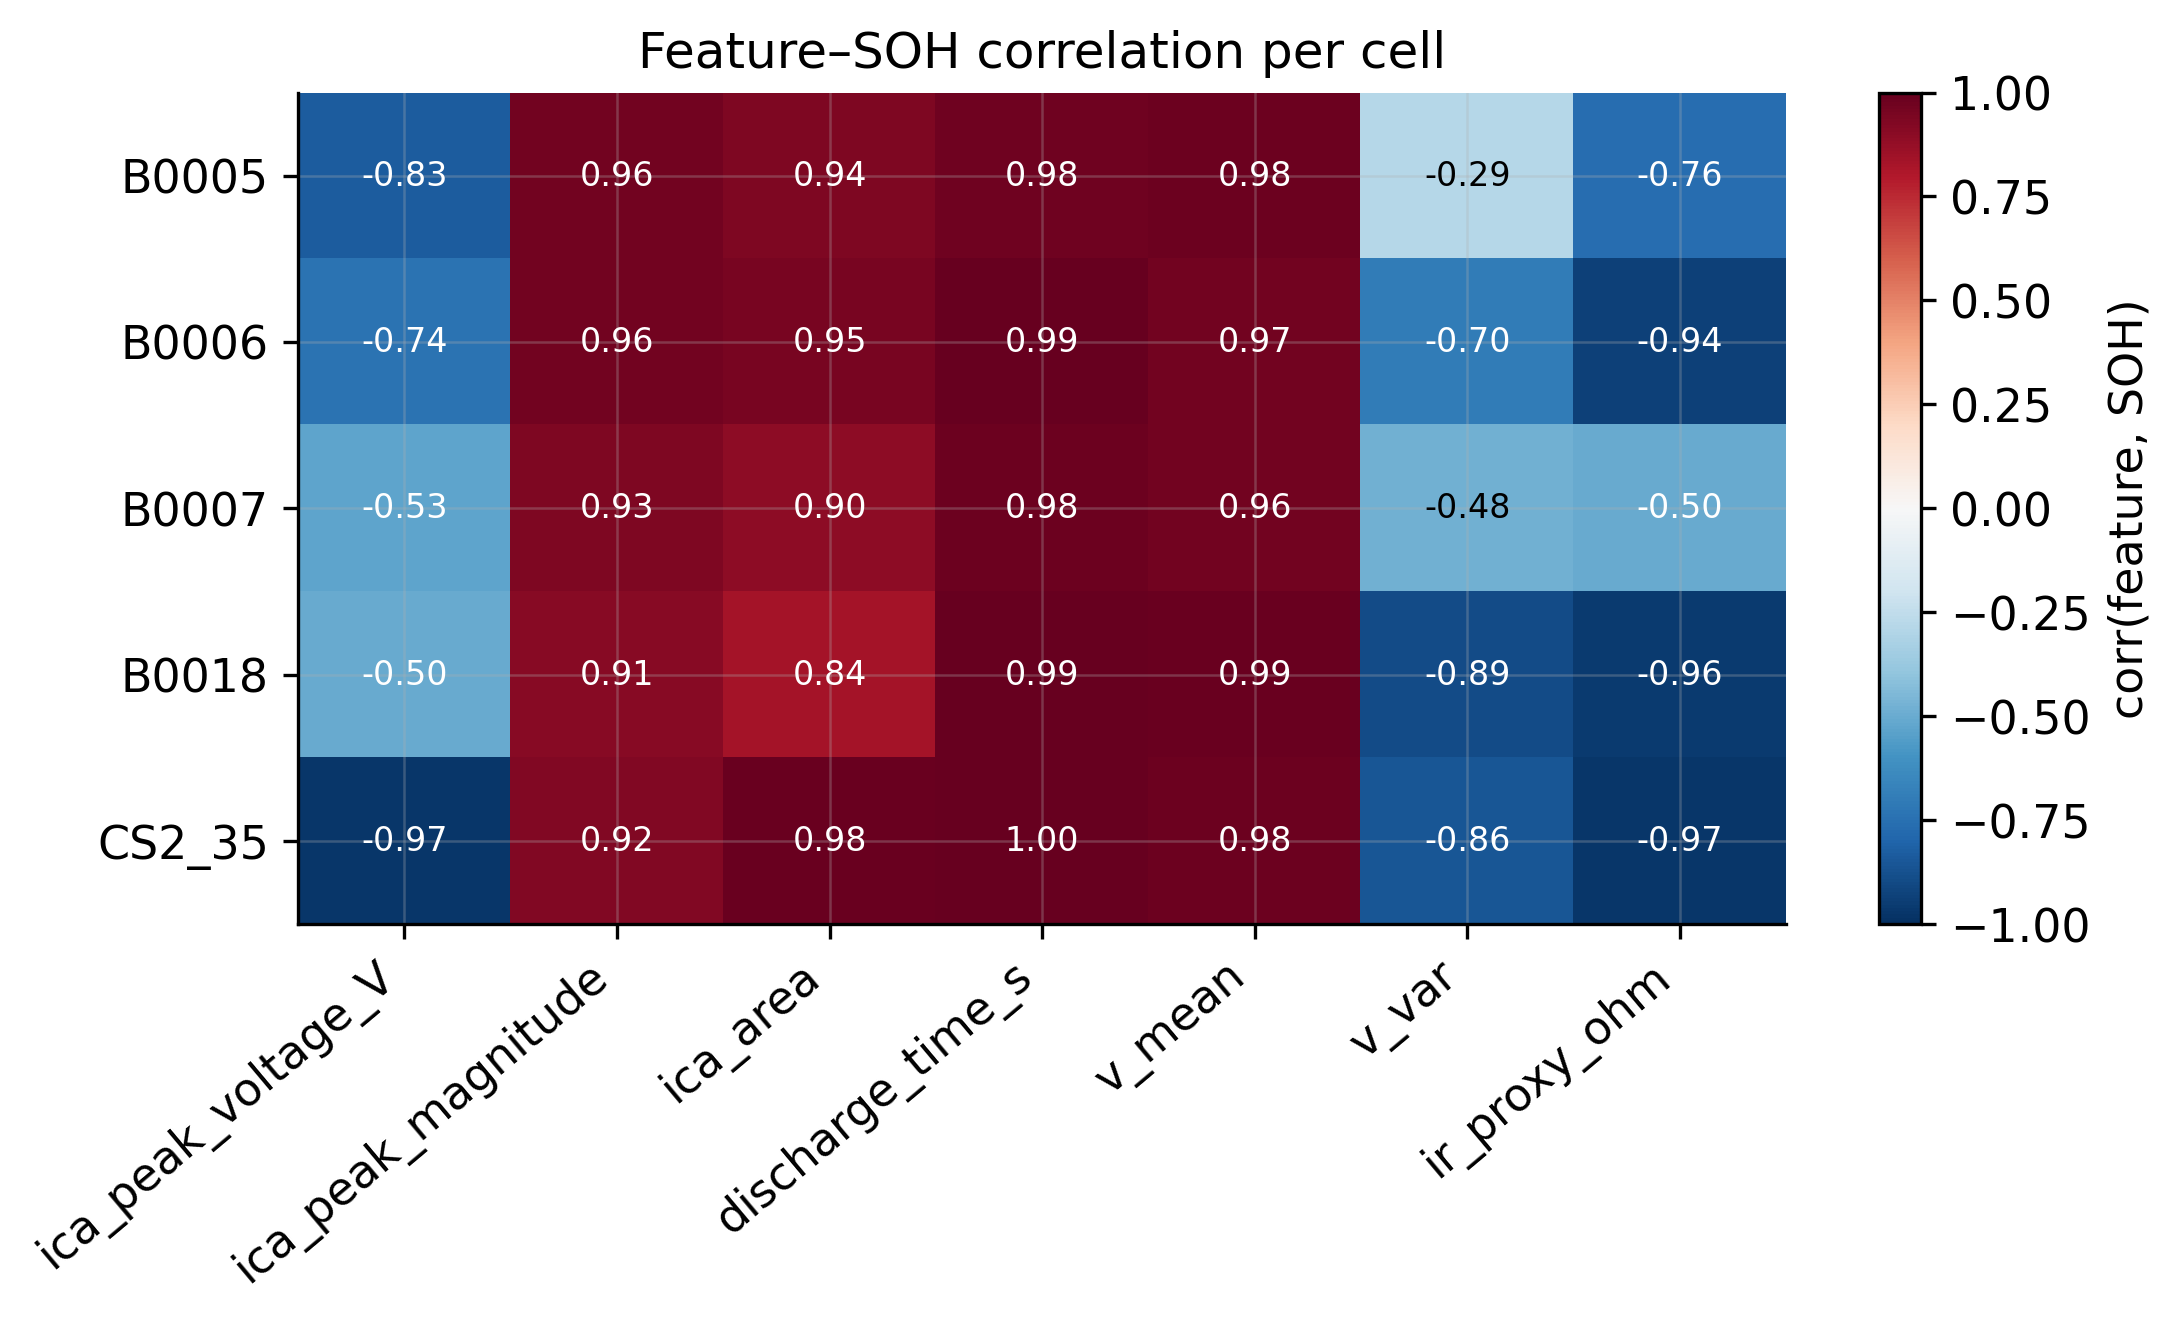
\includegraphics[width=0.85\textwidth]{2-mainmatter/chapters/feature_soh_correlation.png}
    \caption{Per-cell correlation between each engineered feature and SOH. The ICA
    magnitude, ICA area, discharge time and mean voltage are near-perfectly
    correlated with health across all NASA cells and CALCE CS2\_35, while
    intra-cycle voltage variance and the IR proxy carry complementary (negative)
    information.}
    \label{fig:feature_corr}
\end{figure}
\subsubsection{1. NASA PCoE Dataset Diagnostics}
This dataset represents lithium-ion batteries run through continuous
charge/discharge cycles at room temperature until end-of-life (EOL). The
\texttt{.mat} files are parsed directly; charge and discharge half-cycles
alternate, and per-cycle capacity is taken from the discharge phase.
\begin{itemize}
    \item \textbf{Cycle counts (measured):} B0005/B0006/B0007 each yield 168
    aligned cycles and B0018 yields 132, aggregated from tens of thousands of raw
    per-second timeseries points per cell.
    \item \textbf{Target Variables (Labels):}
    \begin{itemize}
        \item \texttt{capacity\_Ah}: per-cycle discharge capacity. Measured initial
        values are 1.856 / 2.035 / 1.891 / 1.855~Ah (B0005/06/07/18); note B0006
        \emph{exceeds} its 2.0~Ah rating at $t_0$.
        \item \textbf{Regeneration is retained in the target:} the localized
        capacity ``bumps'' (B0005 shows 36 such jumps) are \emph{not} smoothed
        away: models are trained and scored against the measured capacity, so
        physical consistency is tested against real regeneration rather than a
        pre-smoothed label. Savitzky--Golay smoothing is used only inside the
        ICA feature extraction and for visualisation.
        \item \textbf{SOH:} $Q/Q_\text{rated}$ with $Q_\text{rated}=2.0$~Ah, giving
        initial SOH 92.8\% (B0005), 101.8\% (B0006), 94.6\% (B0007), 92.8\%
        (B0018). Under this convention, values above 100\% at $t_0$ are
        retained rather than clipped.
    \end{itemize}
    \item \textbf{Engineered predictor features:} the shared eight-feature set
    (ICA peak voltage/magnitude/area, discharge time, $v_\text{min}$,
    $v_\text{mean}$, intra-cycle voltage variance, IR proxy) plus a NASA-only
    temperature-rise feature. Three NASA charge cycles with corrupted voltage logs
    (B0005/06/07 cyc.~32; B0018 cyc.~46,57) are flagged but not dropped.
    \item \textbf{Regeneration:} the localized capacity ``healing'' that a naive
    data-driven model may mistake for genuine recovery is shown for B0005 in
    Figure~\ref{fig:nasa_regen} (36 jumps, the largest 0.088~Ah).
\end{itemize}
\vspace{0.5cm}
\begin{figure}[H]
    \centering
        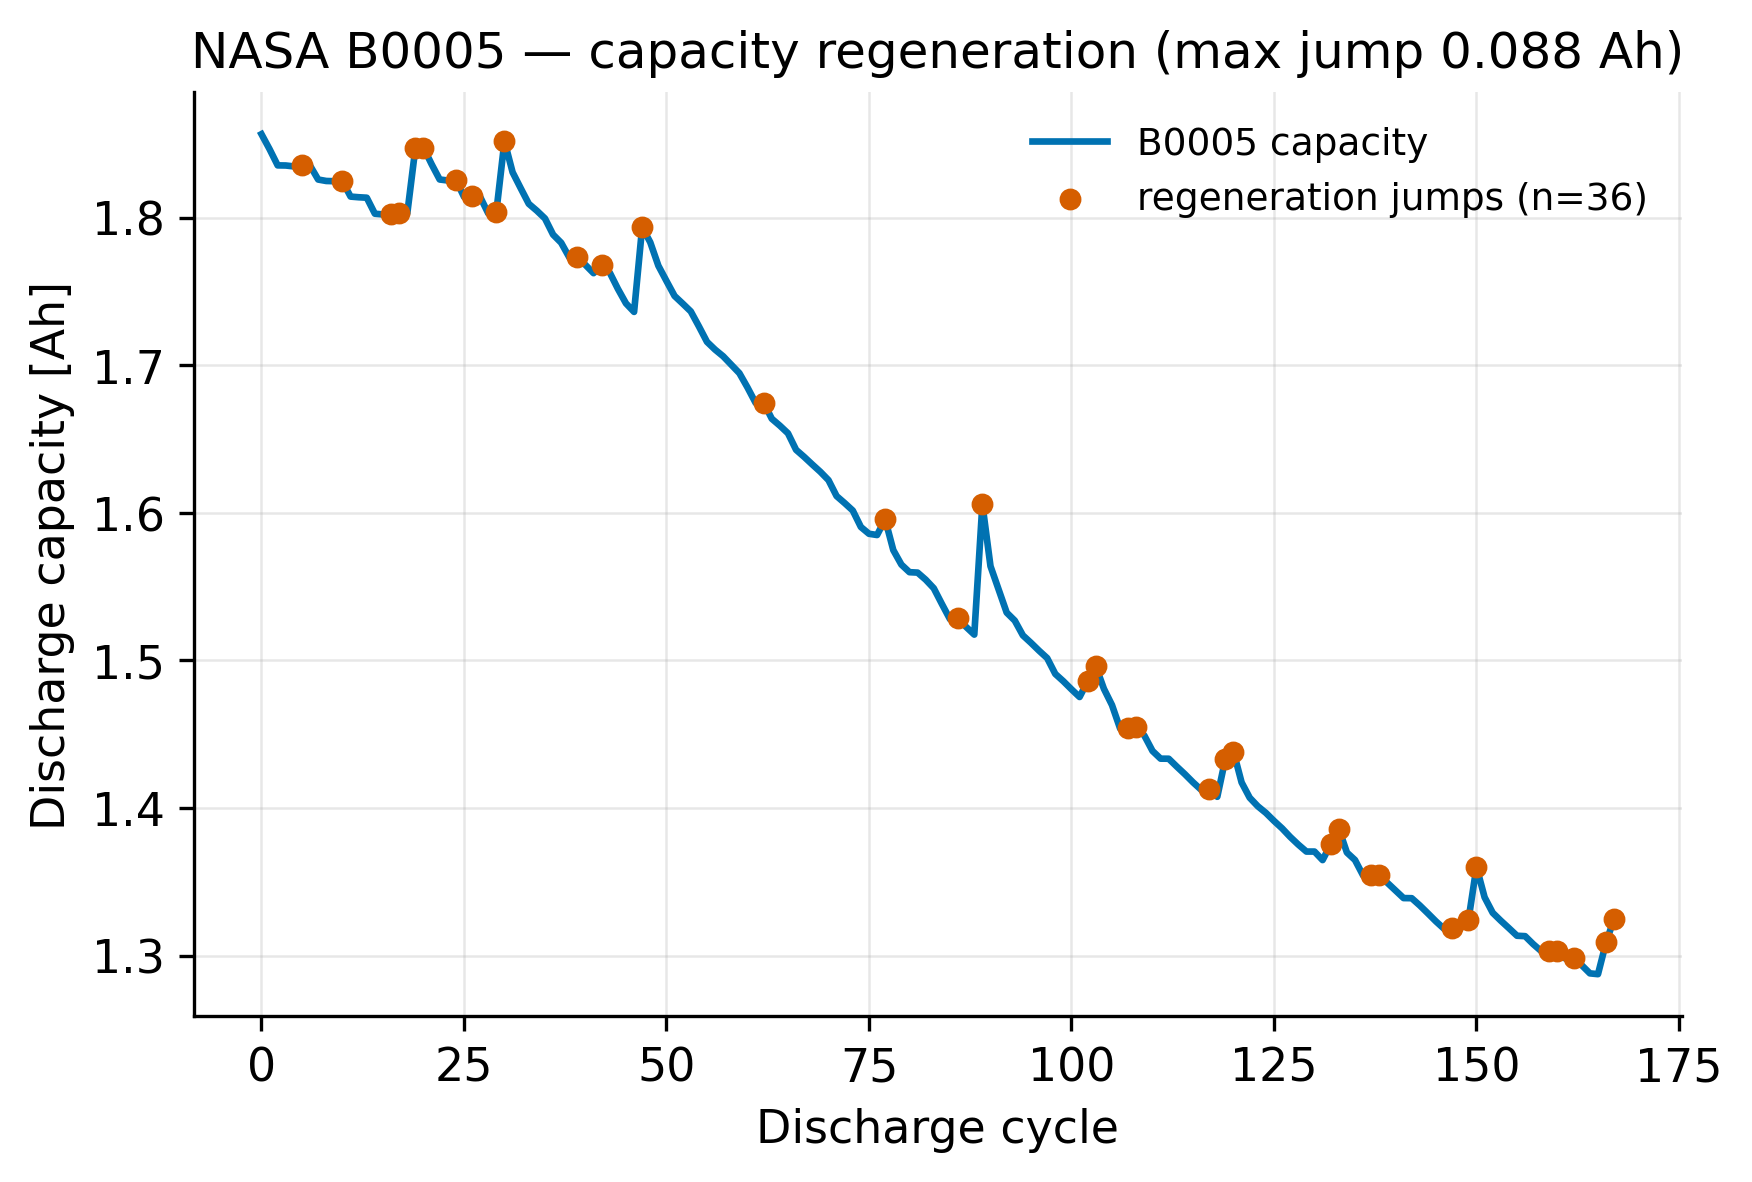
\includegraphics[width=0.8\textwidth]{2-mainmatter/chapters/nasa_b0005_regeneration.png}
    \caption{NASA B0005 capacity with detected regeneration jumps (markers). These
    upward ``healing'' artifacts violate monotonic degradation and motivate the
    physics-consistency constraint enforced by the hybrid model.}
    \label{fig:nasa_regen}
\end{figure}

\subsubsection{2. CALCE Dataset Diagnostics}
This dataset tracks the degradation of a single battery entity (CS2\_35) over a
prolonged period, constructed by chronologically stitching together multiple
individual test files (sorted by their internal \texttt{Date\_Time}, not by
filename).
\begin{itemize}
    \item \textbf{Battery Cell:} CS2\_35, the \texttt{channel\_full} timeline (878
    cycles from 2010-08-16 to early 2011). A byte-identical duplicate file
    (\texttt{CS2\_35\_2\_10\_11}, md5-identical to \texttt{2\_4\_11}) was detected
    and dropped.
    \item \textbf{Record count (measured):} \textbf{260{,}931} raw Channel records.
    (An earlier ``266{,}914'' figure double-counts the duplicate file, and an
    earlier ``160{,}616'' figure is incomplete.)
    \item \textbf{Per-cycle capacity:} computed as the \emph{increment} of the
    cumulative \texttt{Discharge\_Capacity} within the discharge step
    ($\max-\min$), not its maximum. Initial capacity is $\approx1.14$~Ah (the
    $\approx0.88$~Ah quoted earlier is a \emph{mid-life} value, not the initial).
    The raw and Savitzky--Golay-smoothed trajectories are shown in
    Figure~\ref{fig:calce_smoothed}.
    \item \textbf{Engineered predictor features:} the same shared feature set as
    NASA, with ICA peaks extracted via $dQ/dV$ on the CC-charge phase followed by
    Savitzky--Golay smoothing (window~11, polyorder~3), plus a directly measured
    \texttt{internal\_resistance\_Ohm}.
    \item \textbf{Data Quality Note:} the raw stream contains a small number of
    out-of-range cycles (reference/impedance-tracking profiles). Only \emph{4}
    cycles fell outside the physically plausible $[0.30, 1.30]$~Ah window and were
    filtered; the rest of the long-life trajectory is retained.
\end{itemize}
\vspace{0.5cm}
\begin{figure}[H]
    \centering
        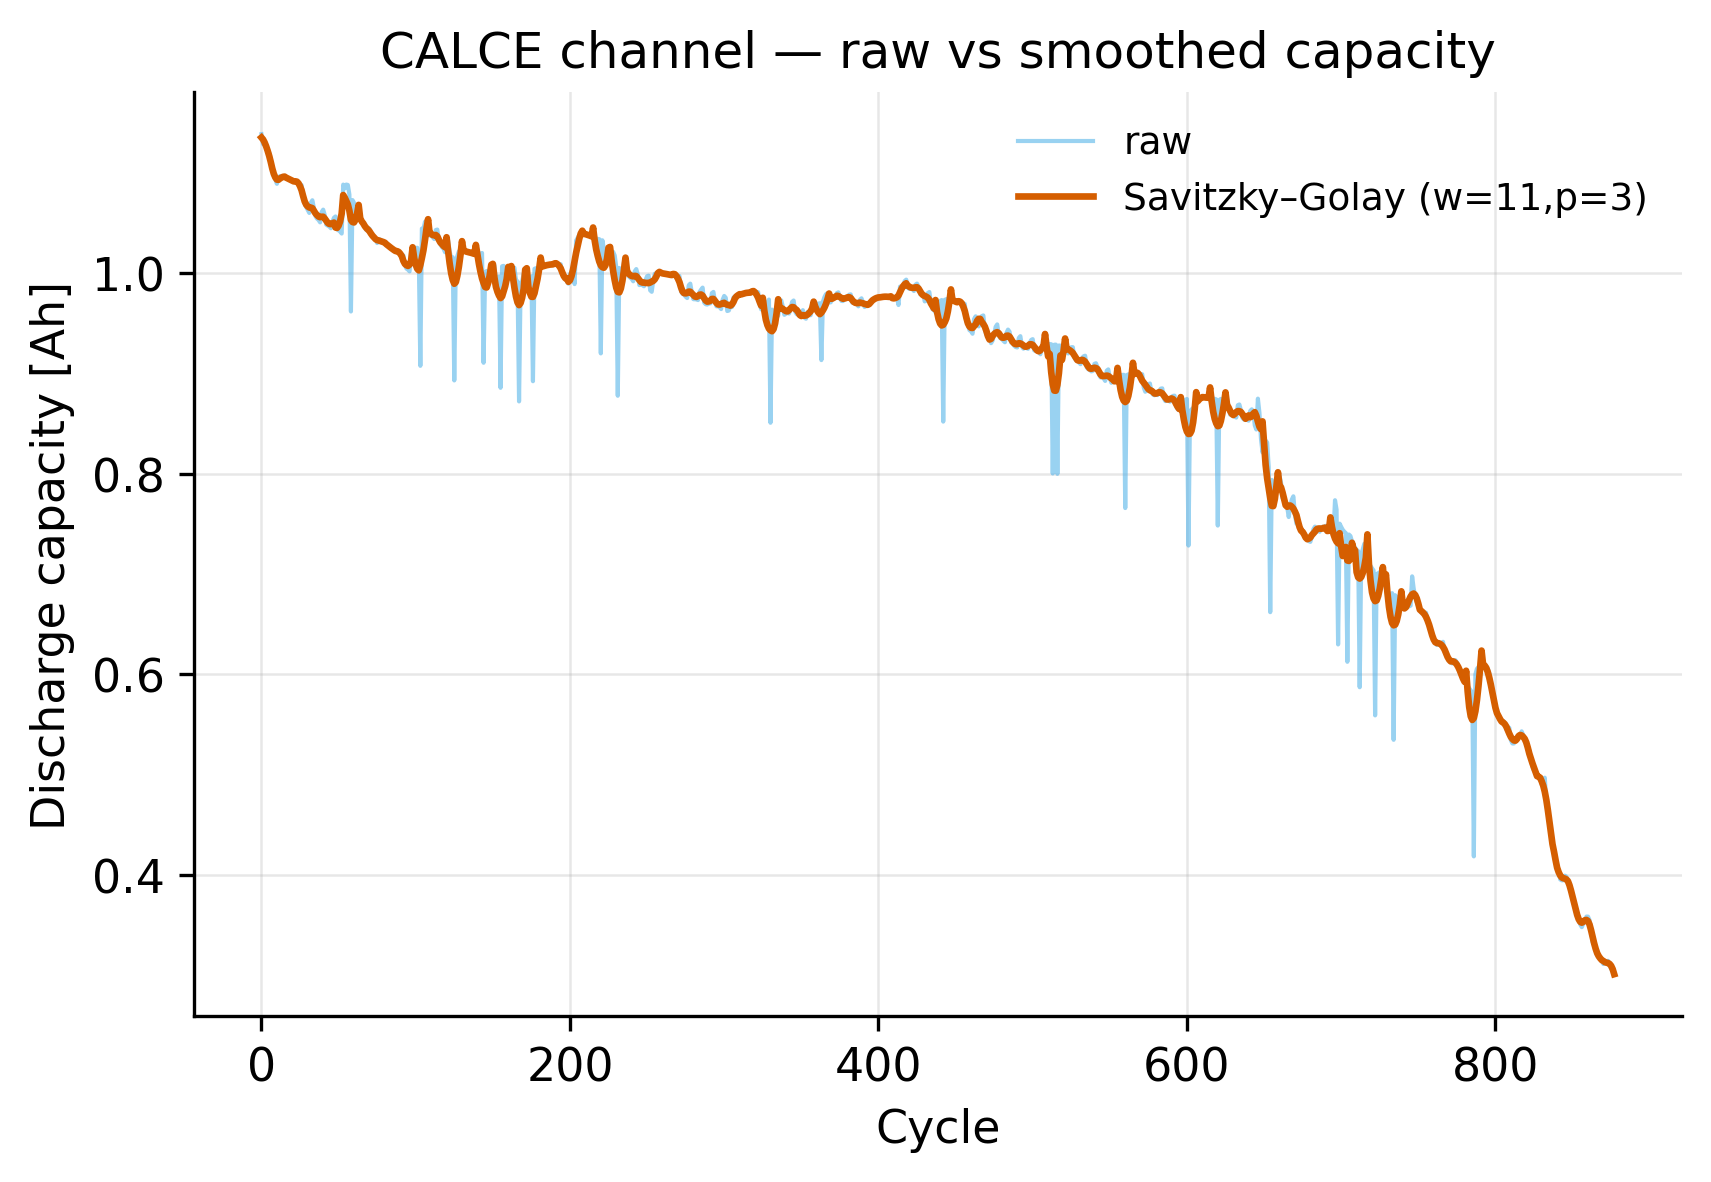
\includegraphics[width=0.8\textwidth]{2-mainmatter/chapters/calce_raw_vs_smoothed.png}
    \caption{CALCE CS2\_35 (\texttt{channel\_full}) raw vs.\ Savitzky--Golay
    smoothed capacity over its full 878-cycle life ($1.14\rightarrow0.30$~Ah). The
    filter (window~11, polyorder~3) removes the sharp downward spikes from
    reference/impedance cycles while preserving the underlying degradation trend.}
    \label{fig:calce_smoothed}
\end{figure}

\begin{figure}[H]
    \centering
        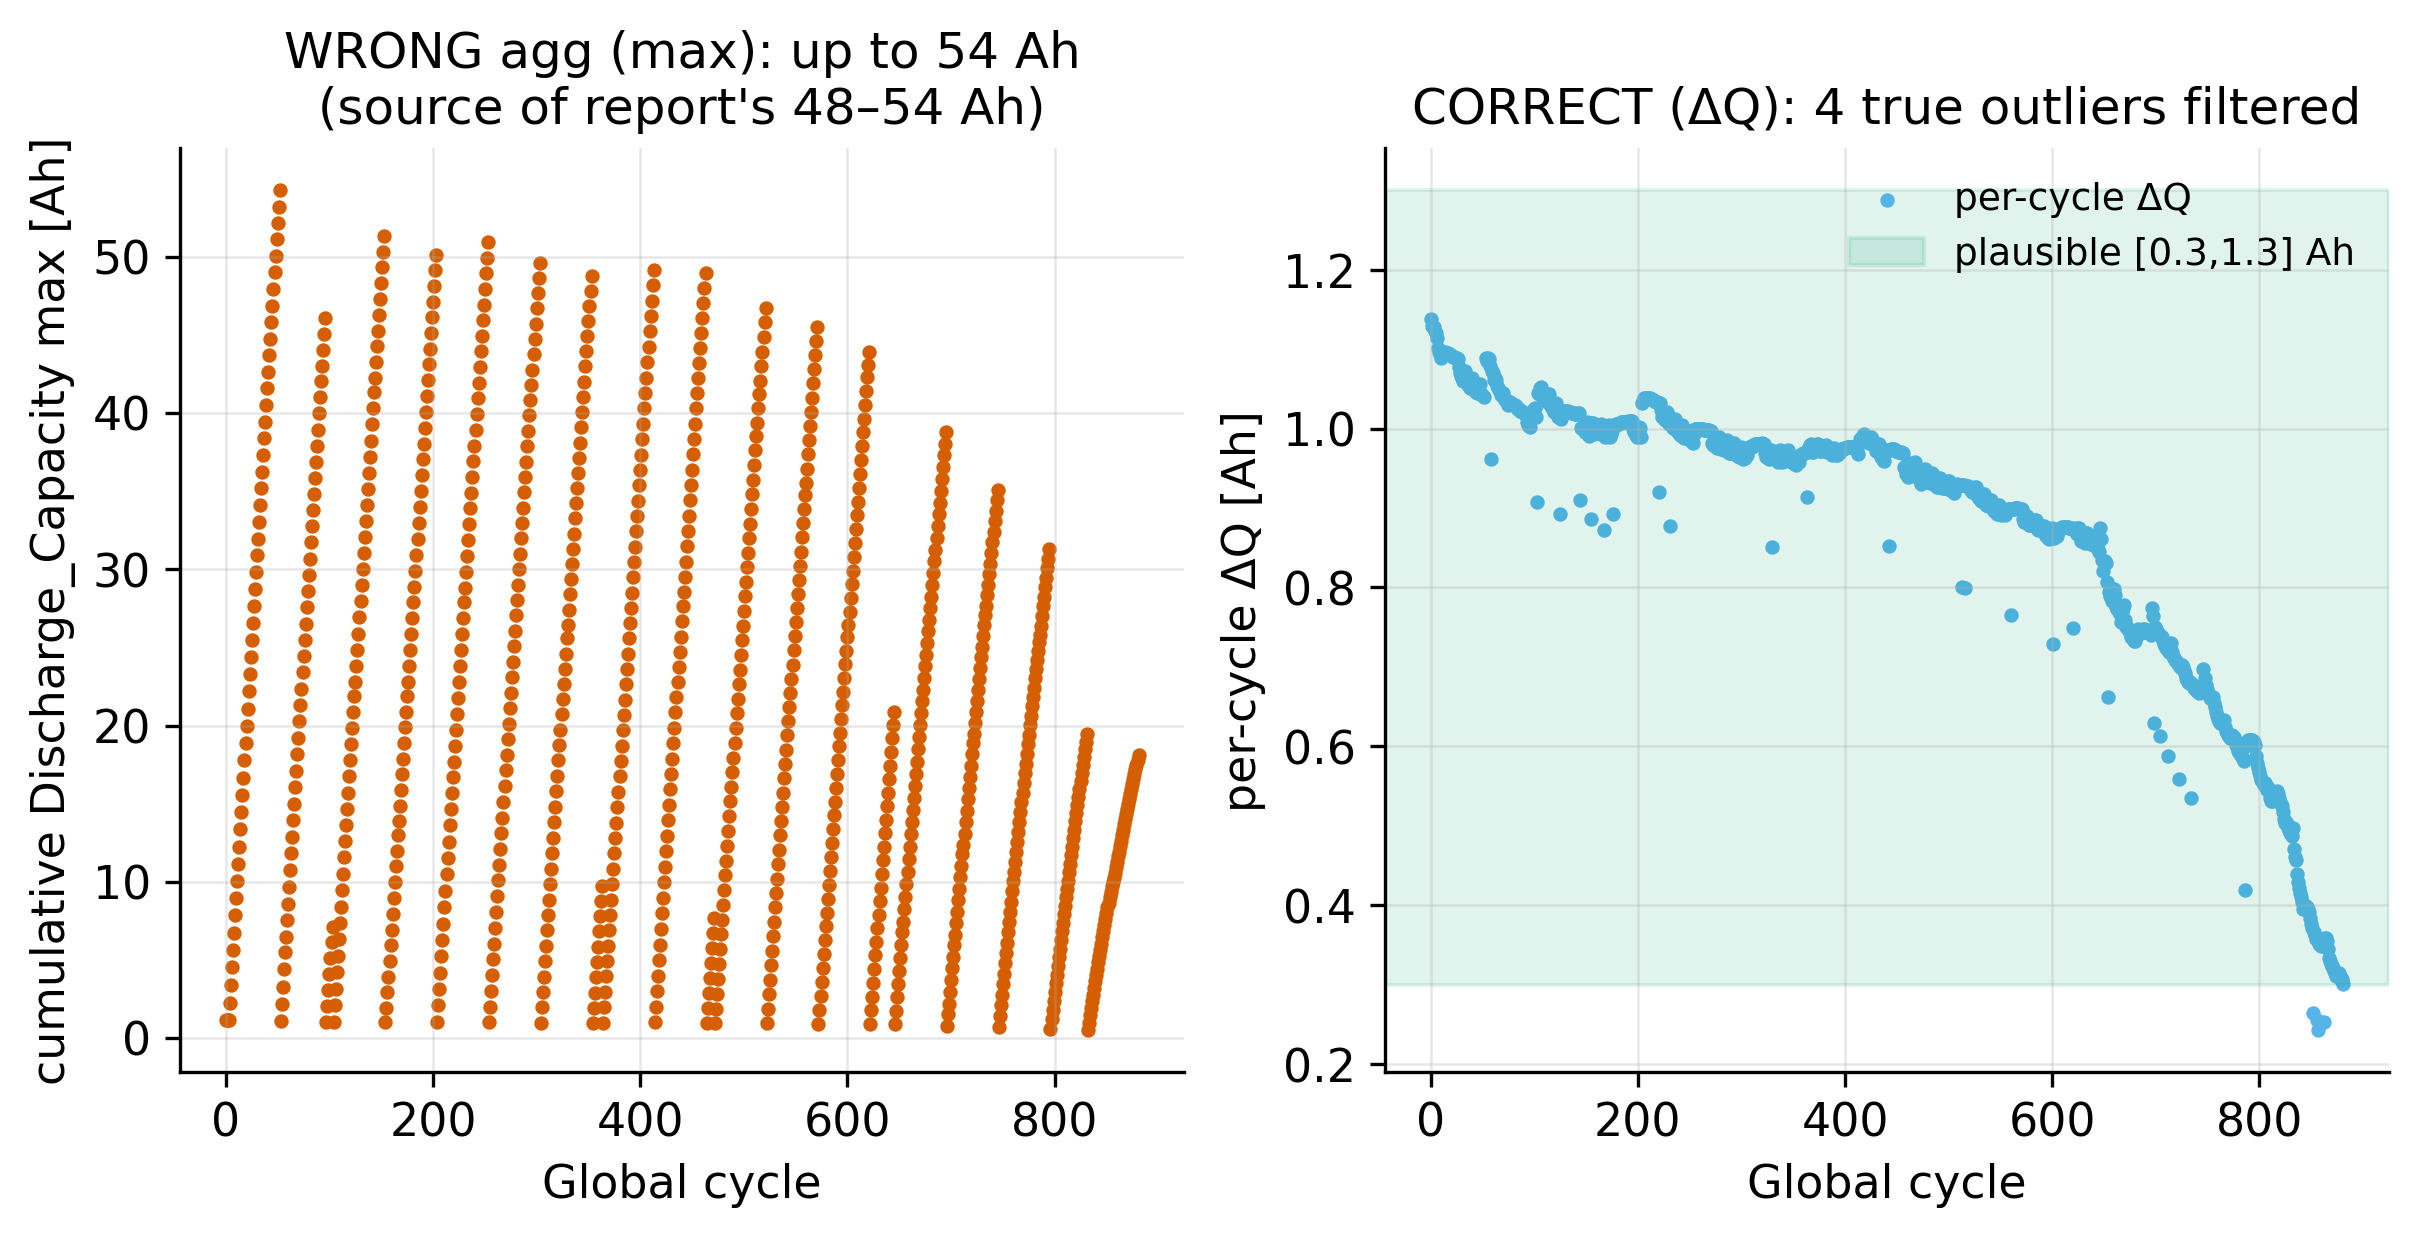
\includegraphics[width=0.95\textwidth]{2-mainmatter/chapters/calce_outliers.png}
    \caption{CALCE capacity extraction. (Left) Taking the \emph{maximum} of the
    cumulative \texttt{Discharge\_Capacity} produces spurious values up to
    $\sim$54~Ah --- the source of the earlier report's ``48--54~Ah'' outliers.
    (Right) The correct per-cycle increment ($\Delta Q$) yields a clean
    degradation curve with only \emph{4} true outliers outside the plausible
    $[0.30,1.30]$~Ah band.}
    \label{fig:calce_outliers}
\end{figure}

\subsubsection{Preprocessing Pipeline Indicators}
Based on the data structures extracted during early implementation phases, the preprocessing pipeline successfully executes four critical transformations:
\begin{enumerate}
    \item \textbf{Chronological Alignment:} Merging separated CALCE date files into a unified, continuous timeline.
    \item \textbf{Temporal Aggregation:} Downsampling high-frequency timeseries data (voltage, current, and temperature recorded per second) into single-cycle statistical summaries (mean, min, variance).
    \item \textbf{Signal Smoothing:} Savitzky--Golay filtering applied to the charge-curve signals \emph{before} the $dQ/dV$ differentiation in the ICA feature extraction (and for trend visualisation). The SOH target itself is deliberately left raw --- see the note above --- so that reported errors reflect the measured degradation.
    \item \textbf{Feature Scaling:} Bounding the features between 0.0 and 1.0 (MinMax scaling) or Standardizing them. This is absolutely critical for the convergence of neural networks and distance-based machine learning baselines.
\end{enumerate}
% --- NEW CONTENT ENDS HERE ---

\section{Evaluation Strategy}
\label{sec:evaluation_strategy}

This section outlines the evaluation protocol to ensure a statistically robust and reproducible assessment of the proposed model.

\subsubsection{Data Splitting and Validation}
To ensure rigorous testing, distinct splitting strategies are employed for the selected datasets:
\begin{itemize}
    \item \textbf{NASA Dataset (B0005, B0006, B0007, B0018):}
    We employ a Leave-One-Cell-Out (LOCO) cross-validation scheme to maximize data
    utility while preventing data leakage. This yields \emph{four} folds: in each
    fold one cell is held out for \emph{test}, a second cell is held out for
    \emph{validation} (early stopping and model selection), and the model is
    trained on the remaining two cells --- whole cells never mix across splits.
    Each fold is repeated over 3 random seeds for stable confidence intervals.
    Scalers and physics priors are fit on the training cells only. In addition
    to the eight engineered features, every learned model receives the same
    fixed-scale normalized cycle coordinate ($\mathrm{cycle}/500$) as an input
    channel: a BMS knows the elapsed cycle count online, and the fixed scale
    carries no information about a trajectory's total recorded length, so the
    input is leak-free and symmetric across models.
    \item \textbf{Cross-Dataset Generalization:}
    To validate the model's ability to handle domain shifts, the model is trained on
    the complete NASA dataset and evaluated directly (zero-shot) on CALCE CS2\_35
    without fine-tuning. As both datasets are LCO, this probes cross-load and
    cross-form-factor robustness rather than cross-chemistry transfer.
\end{itemize}

\subsubsection{Evaluation Metrics}
The predictive performance is quantified using standard regression metrics. For a given cycle $t$:
\begin{align}
\text{MAE}_{SOH} &= \frac{1}{N} \sum_{i=1}^{N} |\widehat{\text{SOH}}_i - \text{SOH}_i|, \\
\text{RMSE}_{SOH} &= \sqrt{ \frac{1}{N} \sum_{i=1}^{N} (\widehat{\text{SOH}}_i - \text{SOH}_i)^2 }, \\
\text{MAE}_{RUL} &= |\widehat{\text{RUL}} - \text{RUL}|.
\end{align}

\noindent
\textbf{Physical Consistency Metric:} To quantify the "physics-informed" advantage, we define a \textbf{Physical Consistency Score (PCS)} which measures the percentage of predictions that respect the monotonic degradation constraint ($d\text{SOH}/dt \le 0$) inherent to battery thermodynamics:
\[
\text{PCS} = \frac{1}{N} \sum_{i=1}^{N} \mathbb{I}\left(\frac{d\widehat{\text{SOH}}}{dt} \le 0\right) \times 100\%
\]
where $\mathbb{I}$ is the indicator function. A higher PCS indicates fewer physical violations (e.g., self-healing artifacts). In implementation, consecutive-cycle increases smaller than $10^{-3}$ SOH are counted as monotone, a numerical tolerance that absorbs floating-point noise without masking real violations. One reference point is essential for reading this metric: because the measured SOH itself contains genuine regeneration, a perfect predictor would \emph{not} score 100\% --- the ground-truth trajectories score PCS 0.847--0.904 on the four NASA cells. PCS is therefore a measure of trend plausibility rather than of accuracy, and a model scoring \emph{above} the ground-truth reference is smoothing through real regeneration transients. For BMS trend estimation this filtering may be acceptable or even desirable, but it is reported as a property, not as an unqualified improvement.

\subsubsection{Statistical Reporting and Ablation}
To ensure scientific rigor, the following protocols are used:
\begin{itemize}
    \item \textbf{Uncertainty Quantification:} Performance is reported as mean $\pm$ 95\% confidence intervals ($1.96\times$ the standard error over folds$\times$seeds).
    \item \textbf{Hypothesis Testing:} Model comparisons use the paired Wilcoxon signed-rank test. Because seeds within a fold share the same test cell, and only four independent cells exist, test outcomes are reported descriptively (fold-level win counts) rather than as strict significance claims (Chapter~\ref{ch:results}).
    \item \textbf{Data Efficiency Study:} the hybrid is compared against the standard baselines on reduced training subsets (25\%, 50\%, 75\%, 100\% of training cycles) to quantify the regularization benefit in data-sparse regimes (results in Chapter~\ref{ch:results}, Section~\ref{sec:ablations}).
\end{itemize}

\section{Benchmarking Baselines}

To satisfy the requirement for rigorous evaluation, the following comparison matrix is established. This selection benchmarks the proposed hybrid framework against pure physics, standard deep learning (LSTM), and high-capacity attention-based models (Transformer).

% --- TABLE 5.2: BENCHMARKS ---
\begin{table}[H]
\centering
\renewcommand{\arraystretch}{1.5} 
\small % Reduces font size slightly to fit more descriptive text
\begin{tabularx}{\textwidth}{@{} >{\raggedright\arraybackslash}p{2.8cm} >{\raggedright\arraybackslash}p{3.2cm} X @{}} 
\toprule
\textbf{Model Category} & \textbf{Specific Algorithm} & \textbf{Role in Research} \\ 
\midrule

\textbf{Empirical} & Double-Exponential Curve Fitting & \textbf{Physical Floor:} Establishes the baseline accuracy of pure curve-fitting. If the hybrid model cannot exceed this, the AI integration adds no value. \\ 

\textbf{Data-Driven (Recurrent)} & Vanilla LSTM / Standard GRU & \textbf{Sequential Control:} Establishes the performance of standard time-series architectures. Comparison isolates the benefit of adding physics-informed loss ($\lambda_{phys} > 0$). \\ 

\textbf{Data-Driven (Classical)} & Support Vector Regression (RBF) & \textbf{Non-Recurrent Control:} A strong shallow regressor on the same windowed features. Isolates the value of \emph{temporal} sequence modelling: if the recurrent networks do not beat it, sequence modelling adds no value on these features. \\

\textbf{Data-Driven (Attention)} & Transformer --- \emph{light} ($\approx$17k params) and \emph{heavy} ($\approx$225k params) & \textbf{Complexity Benchmark:} Two attention scales. The \emph{light} model is edge-sized and hyperparameter-tuned like every baseline; the \emph{heavy} model is a high-capacity accuracy reference at the parameter scale of published attention models, testing whether pure data-driven ``brute force'' can outperform physics-guided learning in data-scarce scenarios. \\

\textbf{Physics-Informed (Alternative)} & Neural-ODE & \textbf{PIML Control:} A continuous-time physics-informed alternative (latent ODE dynamics). Ensures the proposed hybrid is compared against another physics-motivated architecture, not only black boxes. \\

\textbf{Hybrid (Proposed)} & \textbf{Hybrid PINN (Physics-Regularized)} & \textbf{The Solution:} Evaluated on RMSE, data efficiency (25\%--100\% volume), and the ability to maintain physical consistency during extrapolation. \\

\bottomrule
\end{tabularx}
\caption{Benchmark Baselines Comparison Matrix}
\label{tab:benchmarks}
\end{table}
\noindent
Both non-learned floors --- the double-exponential curve fit and the SVR --- are
quantified head-to-head with the neural models in Chapter~\ref{ch:results}
(Table~\ref{tab:benchmark}); the learned models are required to beat them for the
AI component to be justified.
\noindent \textbf{Sufficiency of Data Volume:} While deep learning approaches typically require massive labeled datasets to generalize, \textbf{Physics-Informed models are hypothesised to be data-efficient}: the integration of physical equations constrains the optimization search space, guiding the model even when data is sparse. Rather than assume this, the thesis tests it directly --- via a data-volume ablation on the hybrid and a data-scarcity stress test pitting the hybrid against both Transformer scales at 10--100\% of the training cycles (Chapter~\ref{ch:results}, Sections~\ref{sec:overfitting} and~\ref{sec:ablations}). The combined cycle count of the NASA and CALCE datasets is sufficient for this hypothesis test precisely because the small-data regime is the regime of interest.

\section{Resource Feasibility}

The proposed ``ODE-regularized'' GRU is computationally lightweight. Unlike
PDE-based PINNs which require solving complex spatial grids ($10^5+$ operations),
the added ODE term involves only a few scalar operations (a derivative
calculation). Training is well within the capability of a single GPU or even a
CPU; all results in this thesis were produced on a CPU-only macOS machine.

For real-world BMS deployment, the deployable route-B hybrid is shrunk to a
matched size (hidden $=32$, $\approx$11k parameters) and profiled against the
Cortex-M4 budget. The profiling methodology is stated precisely so that measured
and estimated quantities are never conflated: parameter counts, fp32 model size,
int8 model size (PyTorch dynamic quantisation, qnnpack engine), per-inference
MACs, and peak activation RAM are \emph{measured} on the trained models; only
the Cortex-M4 latency is an analytic MACs-per-clock (CMSIS-NN-style) estimate.
The full footprint table for the hybrid, GRU and both Transformer scales is
reported in Chapter~\ref{ch:results}, Section~\ref{sec:footprint}.

% --- TABLE 5.3: RESOURCE PROFILE ---
\begin{table}[H]
\centering
\caption{Deployment configuration for the lightweight hybrid (parameters, RAM and
MACs measured; int8 size and latency are the clearly-labelled estimates described
above). Full per-model figures appear in Table~\ref{tab:footprint}.}
\label{tab:resource}
\begin{tabularx}{\textwidth}{@{} l X @{}}
\toprule
\textbf{Item} & \textbf{Value (measured)} \\
\midrule
Parameters (matched-size hybrid B, hidden 32) & $\approx$ 11{,}009 \\
Quantized model (int8, flash, measured) & 20.2 KB \\
Runtime activation RAM & 1.25 KB \\
MACs per inference window & $\approx$ 101{,}000 \\
Cortex-M4 latency @ 80 MHz (analytic estimate) & $\approx$ 1.27 ms per window \\
Profiling method & PyTorch dynamic int8 quantisation (qnnpack), measured; analytic latency \\
Training environment & single GPU or CPU (16 GB RAM) \\
\bottomrule
\end{tabularx}
\end{table}

\noindent \textbf{Quantification of Lightweight Architecture:}
The deployable hybrid uses $\approx$11k trainable parameters, comparable to the
small GRU baseline rather than the larger hidden-64 benchmark model, so the
``lightweight'' claim is made on equal footing. After measured int8 quantisation
it occupies \textbf{20.2~KB} of flash and \textbf{1.25~KB} of activation RAM ---
about $3.5\times$ less flash than the light Transformer (70.0~KB / 2.5~KB) and
$30\times$ less than the heavy one (611~KB).

\noindent
Deployment assumptions:
\begin{itemize}
    \item \textbf{Quantization:} 8-bit post-training dynamic quantization
    (PyTorch, qnnpack engine), with the quantised model serialised and its size
    \emph{measured}. Linear and recurrent layers are quantised; attention
    in-projections remain fp32, which is why the Transformers compress by less
    than the ideal $4\times$.
    \item \textbf{Latency:} the Cortex-M4 latency is an analytic MACs/clock
    (CMSIS-NN-style) estimate, clearly labelled as such rather than an on-board
    measurement. On-board validation with a quantised export (ONNX or
    TFLite-Micro) is listed as future work.
\end{itemize}

\noindent
All profiled models fit within standard automotive-MCU constraints
($<$256~KB RAM and $<$1~MB flash) --- the heavy Transformer only after
quantisation, at 60\% of the flash budget, while the deployable hybrid uses
2\% --- confirming that the hybrid approach is feasible for edge deployment.